% !TeX spellcheck = en_us

%-----------------------------------------------------------------------------
%
%               Template for sigplanconf LaTeX Class
%
% Name:         sigplanconf-template.tex
%
% Purpose:      A template for sigplanconf.cls, which is a LaTeX 2e class
%               file for SIGPLAN conference proceedings.
%
% Guide:        Refer to "Author's Guide to the ACM SIGPLAN Class,"
%               sigplanconf-guide.pdf
%
% Author:       Paul C. Anagnostopoulos
%               Windfall Software
%               978 371-2316
%               paul@windfall.com
%
% Created:      15 February 2005
%
%-----------------------------------------------------------------------------


\documentclass[sigconf]{acmart}

% The following \documentclass options may be useful:

% preprint       Remove this option only once the paper is in final form.
%  9pt           Set paper in  9-point type (instead of default 10-point)
% 11pt           Set paper in 11-point type (instead of default 10-point).
% numbers        Produce numeric citations with natbib (instead of default author/year).
% authorversion  Prepare an author version, with appropriate copyright-space text.

%\usepackage[para]{footmisc}
\usepackage[para]{footmisc}
\usepackage{natbib,hyperref}
\usepackage{url}
\usepackage{verbatim}
\usepackage{graphicx}

\newcommand{\cL}{{\cal L}}

\copyrightyear{2018} 
\acmYear{2018} 
%\setcopyright{none} 
\acmConference{COP '18}{July 16, 2018}{Amsterdam, Netherlands}
%\acmDOI{http://dx.doi.org/10.1145/3079368.3079374}
%\acmISBN{978-1-4503-4836-2/17/04}

%\setcopyright{usgov}
%\setcopyright{usgovmixed}
%\setcopyright{cagov}
%\setcopyright{cagovmixed}


% DOI
%\acmDOI{10.475/123_4}

% ISBN
%\acmISBN{123-4567-24-567/08/06}

%Conference
%\acmConference[$\langle$Programming$\rangle$ 2017]{International Conference on the Art, Science, and Engineering of Programming}{April 2017}{Brussels, Belgium} 
%\acmYear{2017}
%\copyrightyear{2017}

%\acmPrice{15.00}


\begin{document}

\special{papersize=8.5in,11in}
\setlength{\pdfpageheight}{\paperheight}
\setlength{\pdfpagewidth}{\paperwidth}


% For compatibility with auto-generated ACM eRights management
% instructions, the following alternate commands are also supported.
%\CopyrightYear{2016}
%\conferenceinfo{CONF'yy,}{Month d--d, 20yy, City, ST, Country}
%\isbn{978-1-nnnn-nnnn-n/yy/mm}\acmPrice{\$15.00}
%\doi{http://dx.doi.org/10.1145/nnnnnnn.nnnnnnn}

% Uncomment the publication rights used.
%\setcopyright{acmcopyright}
\setcopyright{acmlicensed}  % default
%\setcopyright{rightsretained}

%\titlebanner{banner above paper title}        % These are ignored unless
%\preprintfooter{Continuations Code Reviews on any code inside the IDE}   % 'preprint' option specified.

\title{Cross-cutting Commentary}
\subtitle{A Social Coding tool for Modularizing Documentation}

\author{Authors}
%\orcid{1234-5678-9012}
\affiliation{%
  \institution{Hasso Plattner Institute, University of Potsdam}
  \streetaddress{Prof.-Dr.-Helmert-Str. 2-3}
  %\postcode{14482}
  \city{Potsdam} 
  \country{Germany} 
}
\email{email}       
         
\begin{abstract}
Abstract
\end{abstract}

% 2012 ACM Computing Classification System (CSS) concepts
% Generate at 'http://dl.acm.org/ccs/ccs.cfm'.
\begin{CCSXML}<ccs2012>
<concept>
<concept_id>10003120.10003130.10003233</concept_id>
<concept_desc>Human-centered computing~Collaborative and social computing systems and tools</concept_desc>
<concept_significance>500</concept_significance>
</concept>
<concept>
<concept_id>10011007.10011006.10011066.10011069</concept_id>
<concept_desc>Software and its engineering~Integrated and visual development environments</concept_desc>
<concept_significance>300</concept_significance>
</concept>
<concept>
<concept_id>10011007.10011074.10011134</concept_id>
<concept_desc>Software and its engineering~Collaboration in software development</concept_desc>
<concept_significance>100</concept_significance>
</concept>
</ccs2012>
\end{CCSXML}

\ccsdesc[300]{Software and its engineering~Integrated and visual development environments}
\ccsdesc[100]{Software and its engineering~Collaboration in software development}
\ccsdesc[500]{Human-centered computing~Collaborative and social computing systems and tools}
% end generated code

% Legacy 1998 ACM Computing Classification System categories are also
% supported, but not recommended.
%\category{CR-number}{subcategory}{third-level}[fourth-level]
%\category{D.3.0}{Programming Languages}{General}
%\category{F.3.2}{Logics and Meanings of Programs}{Semantics of Programming Languages}[Program analysis]

\keywords{code review, code quality, social coding, feedback}

\maketitle

% !TeX spellcheck = en_us

\section{Introduction}
\begin{enumerate}
	
\item  Problem 1: Reasoning about system is hard\\
Source: General / abstract documentation is either:
\begin{enumerate}
	\item far away from the code (e.g., in wikis or other external documents) => hardly maintained, not directly visible to the developer
	\item or scattered through the code (duplication of documentation) => update anomaly, hard to find all comment instances, 
\end{enumerate}

\item  Problem 2: Finding all code instances for a cross-cutting concern is hard\\
Source: scatted code, not pointers to all code instances



A commentary may be displayed to multiple artifacts, but can have only one location. 
Therefore, the idea is to separate the location from the display of a commentary.


\end{enumerate}


Code comment classification\cite{Pascarella2017ClassifyingCodeComments} 
\section{Background}

\subsection{Code Documentation}

\section{Concept}

\begin{itemize}
\item commentary discusses concerns that cross-cut executable dev. artifacts (e.g., methods, classes)
\item pull comments out of the source code 
\item commentary references development artifacts 
\end{itemize}

\section{Related Work}

\section{Discussion}

\section{Conclusion}

\begin{figure}
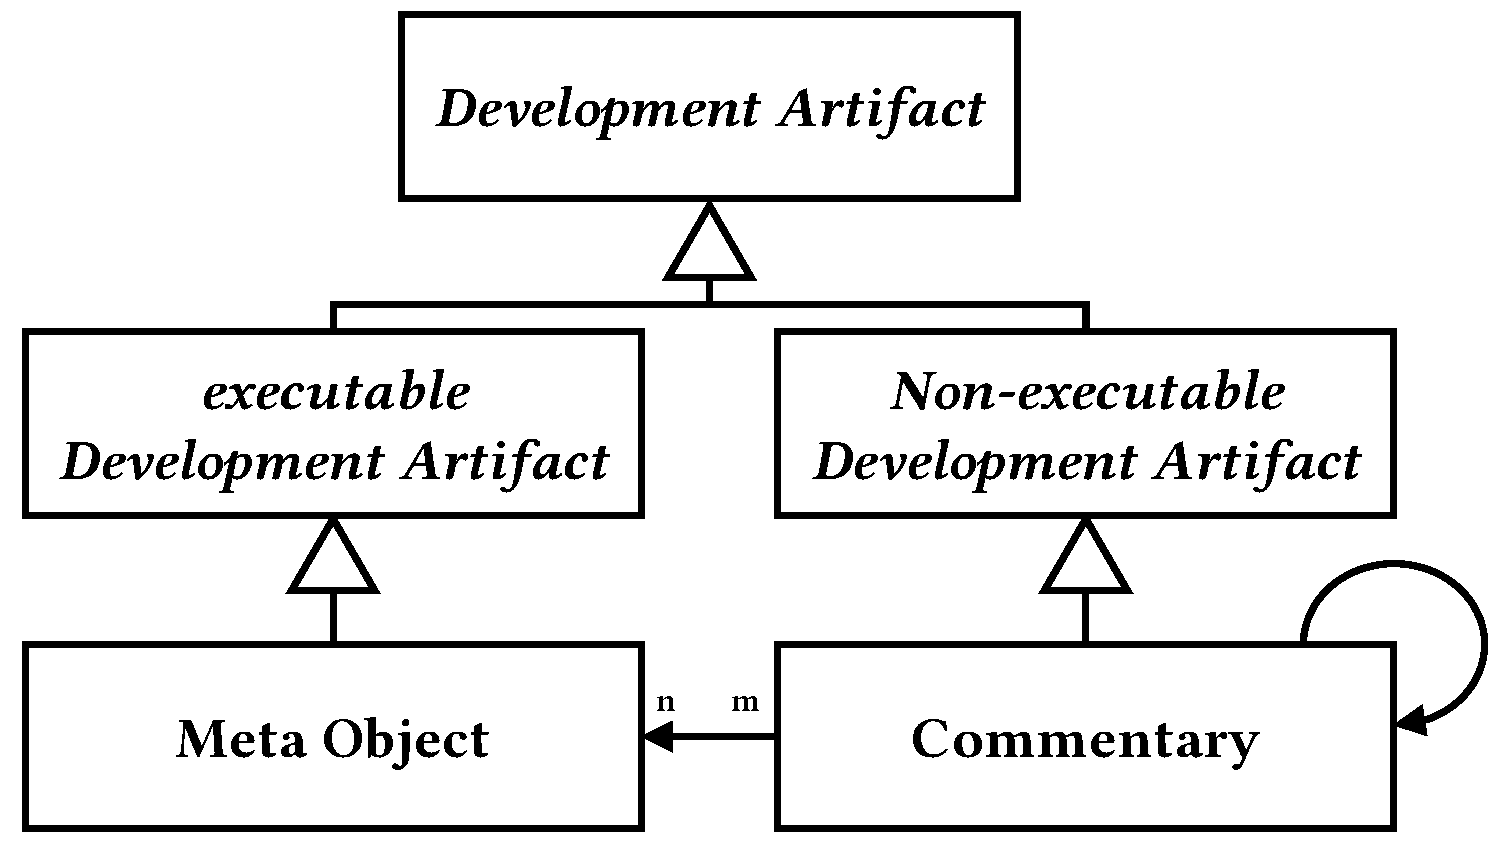
\includegraphics[page=1, width=\columnwidth]{images/metamodel}
\caption{Meta model}
\end{figure}
%\section*{Acknowledgments}

\bibliographystyle{ACM-Reference-Format}
\bibliography{bibliography}

\end{document}

